
\section{density.xml}

The density file contains density constraints for the RBA model.

\subsection{Rationale}

A cell can only contain a limited number of macromolecules:
there is a threshold that the total density
(weight per unit volume) cannot exceed.
Every macromolecule has a weight that equals the sum of its components' weights:

\[
  W_i = \sum_{c \in \mathrm{components}} w_c
\]

If we assign every macromolecule a concentration $C_i$, the total density is:

\[
  \sum_{i \in [1..M]} C_i W_i
\]

where $M$ is the total number of macromolecules.

There are two types of density contraints.
In the first case, the density \emph{must} be equal to some density $d$:

\[
  \sum_{i \in [1..M]} C_i W_i = d
\]

Alternatively, the density must not exceed some maximal density $d_{max}$

\[
  \sum_{i \in [1..M]} C_i W_i \leq d_{max}
\]

The XML format allows for equality and inequality constraints by specifying
whether the bound is a lower bound (not applicable for density),
an upper bound (like $d_{max}$), or a set value (like $d$).

\subsection{RBADensity}
\label{sec:rba_density}

The outermost part of the density file is an instance of class
\rbadensity, shown in Figure~\ref{fig:density_doc}.

\begin{figure}
  \centering
  \includegraphics[scale=0.8]{figures/density_doc}
  \caption{XML structure of density document.}
\label{fig:density_doc}
\end{figure}

\rbadensity{} has no simple attributes.
It includes exactly one instance of \textbf{ListOf} container classes.
All \textbf{ListOf} classes do not have own attributes,
they are merely used to organize a list of instances from another class.

\subsection{TargetDensity}
\label{sec:target_density}

The \targetdensity{} class is used to define density constraints
(Fig.~\ref{fig:density_doc}).
In a RBA model, a density constraint defines how many molecules
a given compartment can contain.
It inherits \targetvalue{} for the constraint definition part.

\paragraph{The \textit{compartment} attribute}
The \textbf{compartment} attribute must match the identifier of a \compartment.


\subsection{TargetValue}
\label{sec:target_value}

The \targetvalue{} class is used to define the sign of an additional RBA
constraint and the value of its second member
(Fig.~\ref{fig:density_doc}).
It is designed to be inherited.
The child class usually holds information about the first member of the
constraint
(\textit{e.g.} compartment for a density constraint,
metabolite for a production constraint).

\paragraph{The \textit{value}, \textit{lowerBound} and \textit{upperBound} attributes}
Every attribute can be left undefined, or
contain the identifier of a \function{} or an \aggregate.

If \textbf{value} is defined, the constraint is an equally constraint.
\textbf{lowerBound} and \textbf{upperBound} are ignored.
If \textbf{value} is undefined, \textbf{lowerBound} (resp. \textbf{upperBound}) defines
a lower bound (resp.\ upper bound) inequality constraint.
Note that \textbf{lowerBound} and \textbf{upperBound} may both be defined, yielding two
separate inequality constraints.

\subsection{Examples}

density.xml is by far the shortest file in an RBA model
(Fig.~\ref{fig:density_ex_1} and \ref{fig:density_ex_2}).
Usually it contains one constraint per compartment,
even though there may be zero or more than one constraint per compartment.
In general, we advise using inequality constraints for greater flexibility
in the model.

\begin{figure}
  \centering
  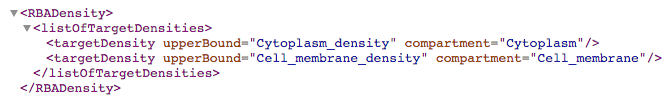
\includegraphics[scale=0.6]{figures/density_ex_1}
  \caption{density.xml from a hand-curated model for the
  model bacteria \textit{B. subtils}.
  The model defines two density constraints, one per compartment.
  By using upperBound, we define two inquality constraints:
  the density of macromolecules may not exceed parameter
  Cytoplasm\_density in the cytoplasm or Cell\_membrane\_density in the membrane,
  but any lower value is acceptable.}
  \label{fig:density_ex_1}
\end{figure}

\begin{figure}
  \centering
  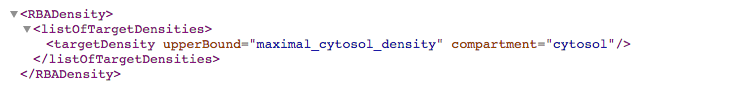
\includegraphics[scale=0.6]{figures/density_ex_2}
  \caption{density.xml from the minimal model.
  There is only one compartment in the minimal model,
  for which we define an upperBound type density constraint.}
  \label{fig:density_ex_2}
\end{figure}
